%%%%%%%%%%%%%%%%%%%%%%%%%%%%%%%%%%%%%%%%%%%%%%%%%%%%%%%%%%%%%%%%%%%%%%%%%%%%%%%%%%
\begin{frame}[fragile]\frametitle{}
\begin{center}
{\Large Overview}
\end{center}
\end{frame}

%%%%%%%%%%%%%%%%%%%%%%%%%%%%%%%%%%%%%%%%%%%%%%%%%%%%%%%%%%%
\begin{frame}[fragile]\frametitle{Overview of Prompt Engineering}

\begin{itemize}
  \item \textbf{Introduction}
    \begin{itemize}
      \item Large Language Models (LLMs) differ from traditional ML models.
      \item LLMs provide unique insights without requiring retraining.
    \end{itemize}
  
  \item \textbf{Transformational Impact}
    \begin{itemize}
      \item LLMs have catalyzed a transformative wave in programming.
      \item Enables effortless computer programming through simple text prompts.
    \end{itemize}

  \item \textbf{Prompt Engineering Technique}
    \begin{itemize}
      \item Technique for directing LLM responses without altering model weights.
      \item Relies on strategic in-context prompting.
      \item Art of effectively communicating with AI for desired outcomes.
    \end{itemize}
  
  \item \textbf{Application Spectrum}
    \begin{itemize}
      \item Applied across various tasks: question-answering, arithmetic reasoning, etc.
      \item Serves as a versatile tool to explore LLM boundaries and potentials.
    \end{itemize}
\end{itemize}

\end{frame}

%%%%%%%%%%%%%%%%%%%%%%%%%%%%%%%%%%%%%%%%%%%%%%%%%%%%%%%%%%%
\begin{frame}[fragile]\frametitle{Progression}

Models for prediction:

\begin{itemize}
\item On data, derive features, put statistical techniques like regression. One model per task. That's Machine Learning.
\item Feed raw data, employ neural networks. One model per task. That's Deep Learning.
\item Use Text data, get embeddings, use ML/DL, say for classification. One model per task. That's Natural Language Processing.
\item Train neural network on large corpus, store weights and architecture, then add final layers for say classification on custom data+labels. That's Pretrained model. One model, many tasks.
\item Train Large Language Model, just supply instructions on what to do, works. One model many tasks. Zero-shot, few-shots.
\end{itemize}

{\tiny (More info at SaaS LLM https://medium.com/google-developer-experts/saasgpt-84ba80265d0f)}

\end{frame}


%%%%%%%%%%%%%%%%%%%%%%%%%%%%%%%%%%%%%%%%%%%%%%%%%%%%%%%%%%%
\begin{frame}[fragile]\frametitle{New Programming Language?}

\begin{center}

\includegraphics[width=0.8\linewidth,keepaspectratio]{promptengg1}

{\tiny (Ref: Prompt Engineering Sudalai Rajkumar)}

\end{center}				

\end{frame}



%%%%%%%%%%%%%%%%%%%%%%%%%%%%%%%%%%%%%%%%%%%%%%%%%%%%%%%%%%%
\begin{frame}[fragile]\frametitle{What is Prompt Engineering?}

Prompt engineering is a NLP concept that involves discovering inputs that yield desirable or useful results


\begin{center}
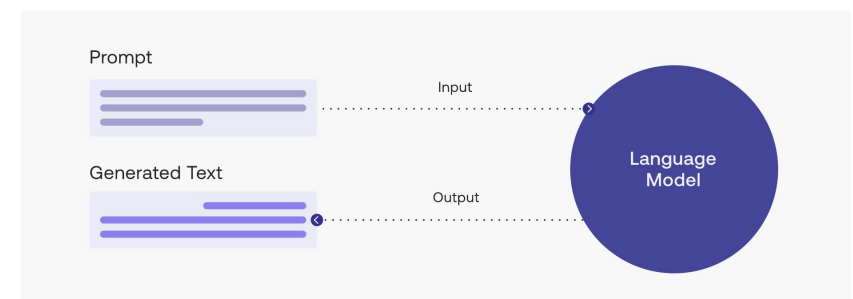
\includegraphics[width=\linewidth,keepaspectratio]{promptengg2}

{\tiny (Ref: Cohere https://docs.cohere.ai/docs/prompt-engineering)}

\end{center}				
			
			

\end{frame}



%%%%%%%%%%%%%%%%%%%%%%%%%%%%%%%%%%%%%%%%%%%%%%%%%%%%%%%%%%%
\begin{frame}[fragile]\frametitle{What is a Language Models?}

\begin{itemize}
\item While typing SMS, have you seen it suggests next word?
\item While typing email, have you seen next few words are suggested?
\item How does it suggest? (suggestions are not random, right?)
\item In the past, for ``Lets go for a \ldots', if you have typed 'coffee' 15 times, 'movie' say 4 times, then it learns that. Machine/Statistical Learning.
\item Next time, when you type ``Lets go for a '', what will be suggested? why?
\item This is called Language Model. Predicting the next word. When done continuously, one after other, it spits sentence, called Generative Model.
\end{itemize}	

\begin{center}
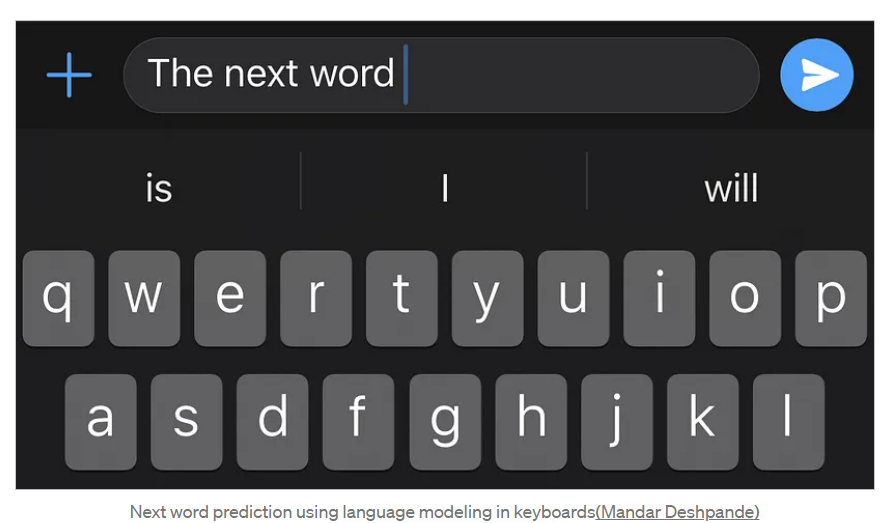
\includegraphics[width=0.6\linewidth,keepaspectratio]{chatgpt34}
\end{center}		

\end{frame}

%%%%%%%%%%%%%%%%%%%%%%%%%%%%%%%%%%%%%%%%%%%%%%%%%%%%%%%%%%%
\begin{frame}[fragile]\frametitle{Evolution of Language Models}

Language Models can be statistical (frequency based) or Machine/Deep Learning (supervised) based. Simple to complex.

\begin{center}
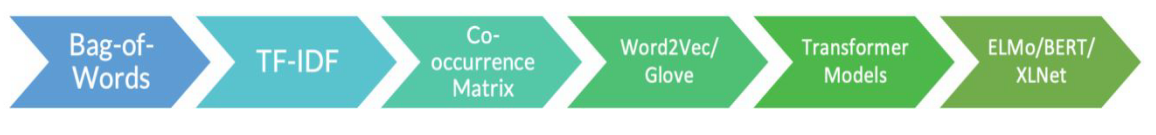
\includegraphics[width=\linewidth,keepaspectratio]{chatgpt30}
\end{center}				
{\tiny (Ref: Analytics Vidhya https://editor.analyticsvidhya.com/uploads/59483evolution\_of\_NLP.png)}

\end{frame}

%%%%%%%%%%%%%%%%%%%%%%%%%%%%%%%%%%%%%%%%%%%%%%%%%%%%%%%%%%%
\begin{frame}[fragile]\frametitle{Large Language Models - Comparison}

\begin{center}
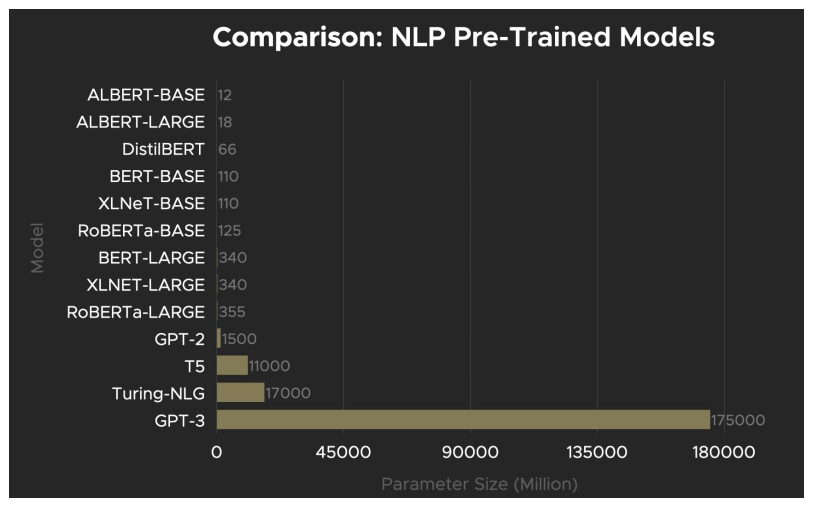
\includegraphics[width=\linewidth,keepaspectratio]{chatgpt31}
\end{center}				
{\tiny (Ref: Deus.ai https://www.deus.ai/post/gpt-3-what-is-all-the-excitement-about)}

\end{frame}


%%%%%%%%%%%%%%%%%%%%%%%%%%%%%%%%%%%%%%%%%%%%%%%%%%%%%%%%%%%
\begin{frame}[fragile]\frametitle{What is Prompt Engineering?}

\begin{itemize}
\item For prompt \lstinline|What is 1,000,000 * 9,000?| GPT-3 (text-davinci-002) (sometimes) answers 9,000,000 (incorrect). This is where prompt engineering comes in.
\item If, instead of asking What is \lstinline|1,000,000 * 9,000?|, we ask \lstinline|What is 1,000,000 * 9,000? Make sure to put the right amount of zeros, even if there are many:|, GPT-3 will answer 9,000,000,000 (correct). 
\item Why is this the case? Why is the additional specification of the number of zeros necessary for the AI to get the right answer? How can we create prompts that yield optimal results on our task? 			
\item That's Prompt Engineering.
\end{itemize}

{\tiny (Ref: https://learnprompting.org/docs/basics/prompting)}
\end{frame}

%%%%%%%%%%%%%%%%%%%%%%%%%%%%%%%%%%%%%%%%%%%%%%%%%%%%%%%%%%%
\begin{frame}[fragile]\frametitle{What is Prompt Engineering?}

How to talk to AI to get it to do what you want


\begin{center}
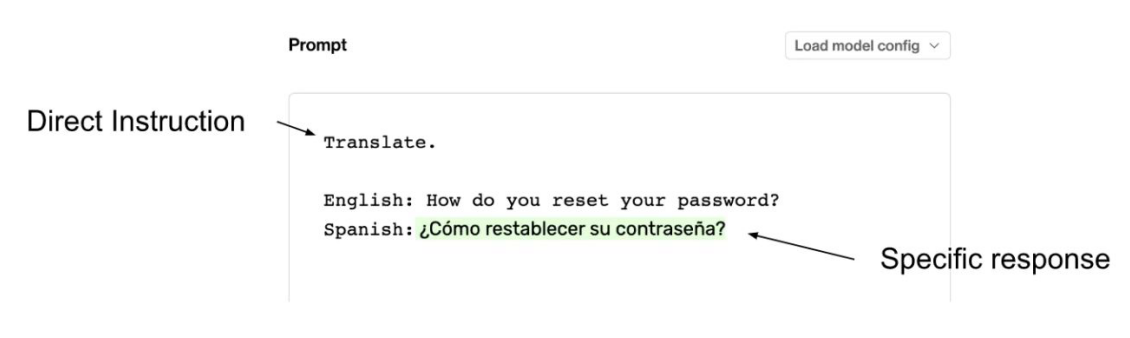
\includegraphics[width=\linewidth,keepaspectratio]{promptengg3}

{\tiny (Ref: Human Loop https://humanloop.com/blog/prompt-engineering-101)}

\end{center}				
			
			

\end{frame}

%%%%%%%%%%%%%%%%%%%%%%%%%%%%%%%%%%%%%%%%%%%%%%%%%%%%%%%%%%%
\begin{frame}[fragile]\frametitle{What is Prompt Engineering?}

But need to tell, for sure, else, nothing


\begin{center}
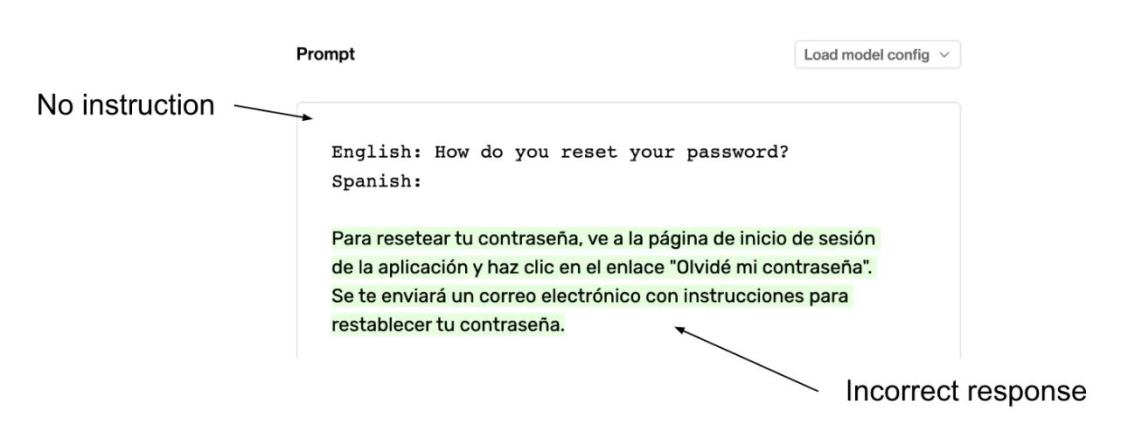
\includegraphics[width=\linewidth,keepaspectratio]{promptengg4}

{\tiny (Ref: Human Loop https://humanloop.com/blog/prompt-engineering-101)}

\end{center}				

\end{frame}



%%%%%%%%%%%%%%%%%%%%%%%%%%%%%%%%%%%%%%%%%%%%%%%%%%%%%%%%%%%%%%%%%%%%%%%%%%%%%%%%%%
\begin{frame}[fragile]\frametitle{}
\begin{center}
{\Large Engineering of Prompts}
\end{center}
\end{frame}

%%%%%%%%%%%%%%%%%%%%%%%%%%%%%%%%%%%%%%%%%%%%%%%%%%%%%%%%%%%
\begin{frame}[fragile]\frametitle{Elements of Prompt}

A prompt is composed of:

\begin{center}
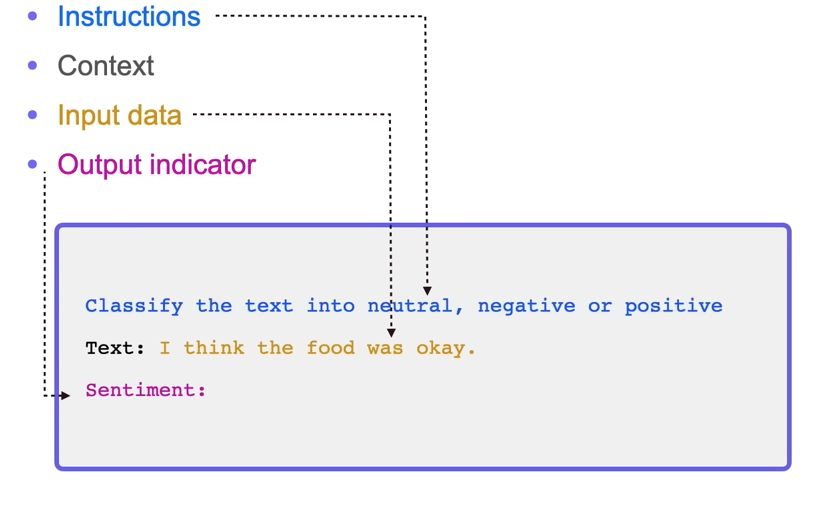
\includegraphics[width=0.8\linewidth,keepaspectratio]{promptengg28}

{\tiny (Ref: Prompt Engineering Overview - Elvis Saravia)}

\end{center}		
		
\end{frame}


%%%%%%%%%%%%%%%%%%%%%%%%%%%%%%%%%%%%%%%%%%%%%%%%%%%%%%%%%%%
\begin{frame}[fragile]\frametitle{Settings of Prompt}

\begin{itemize}
\item 'temperature':  before applying the softmax function, temperature is used scale the logits. With it, creativity or variability is allowed. If you re-run the prompt, with 0, no change, but with 1, lots of variation. Default is 0.7. With a temperature between 0 and 1, we can control the randomness and creativity of the model's predictions. Temperature defines how likely it is to choose less probable words. T=0 gives the same response every time because there's a 0% chance to choose any word but the most likely. T=1 just picks based on the model's base confidence.
\item 'top\_p' or 'nucleus sampling': specifies a sampling threshold during inference time, words passing the threshold are sampled for the output. Top-p goes for a minimal set of words, the probability of which does not exceed exceeds p. In practice, this means the following: if you choose reasonably high p, like 0.9, you would likely get a set of the most likely words for the model to choose from
\item Like the temperature, the top p parameter controls the randomness and originality of the model.
\item OpenAI documentation recommends using either one parameter or the other and setting the unused parameter to the neutral case, i.e. 1.0.
\end{itemize}
		
\end{frame}


%%%%%%%%%%%%%%%%%%%%%%%%%%%%%%%%%%%%%%%%%%%%%%%%%%%%%%%%%%%
\begin{frame}[fragile]\frametitle{Prompting by Instruction}

\begin{center}
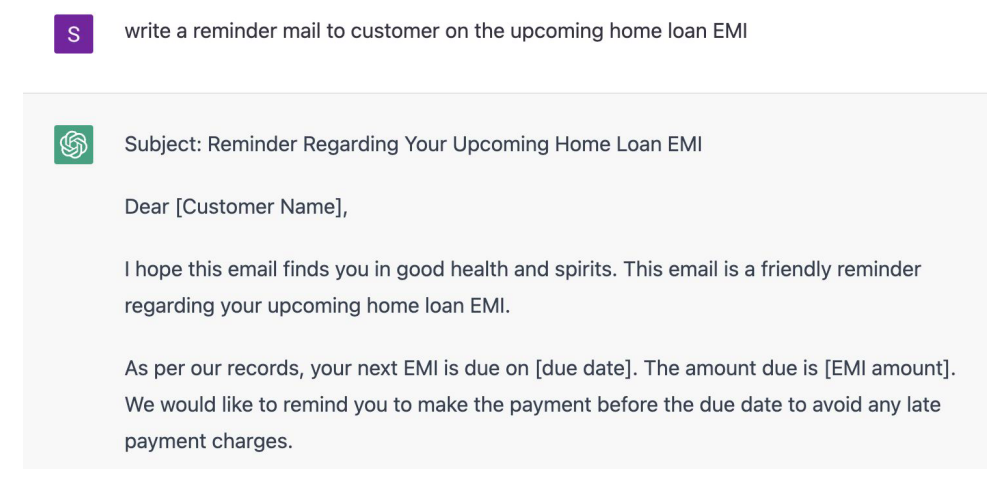
\includegraphics[width=\linewidth,keepaspectratio]{promptengg7}

{\tiny (Ref: Cohere https://txt.cohere.ai/generative-ai-part-1/)}

\end{center}		

\end{frame}



%%%%%%%%%%%%%%%%%%%%%%%%%%%%%%%%%%%%%%%%%%%%%%%%%%%%%%%%%%%
\begin{frame}[fragile]\frametitle{Length Control}

Specify a desired word count or character count as part of the prompt

\begin{center}
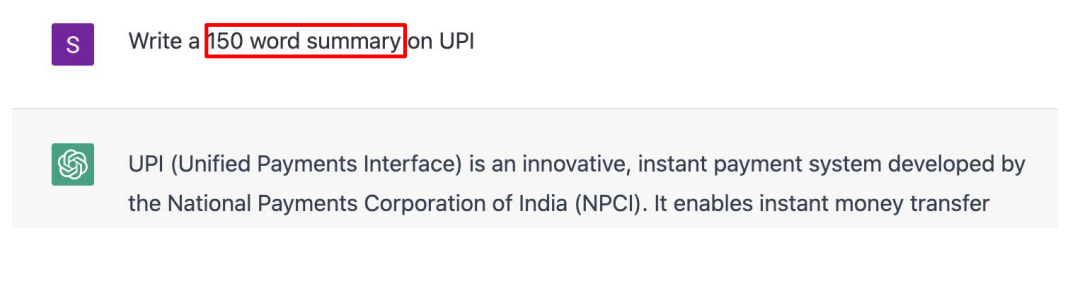
\includegraphics[width=\linewidth,keepaspectratio]{promptengg16}

{\tiny (Ref: Prompt Engineering Sudalai Rajkumar)}

\end{center}		

\end{frame}

%%%%%%%%%%%%%%%%%%%%%%%%%%%%%%%%%%%%%%%%%%%%%%%%%%%%%%%%%%%
\begin{frame}[fragile]\frametitle{Tone Control}

Specify specific words or phrases that indicate the desired tone

\begin{center}
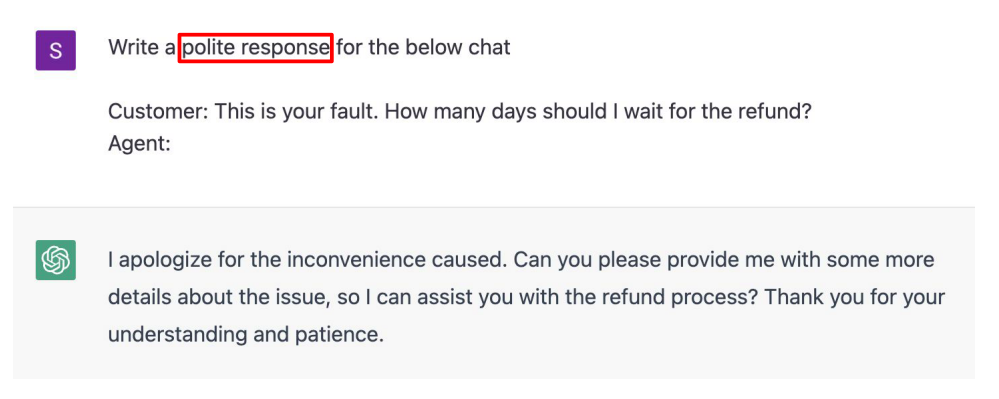
\includegraphics[width=\linewidth,keepaspectratio]{promptengg17}

{\tiny (Ref: Prompt Engineering Sudalai Rajkumar)}

\end{center}		

\end{frame}

%%%%%%%%%%%%%%%%%%%%%%%%%%%%%%%%%%%%%%%%%%%%%%%%%%%%%%%%%%%
\begin{frame}[fragile]\frametitle{Style Control}

Specify the desired writing style.

\begin{center}
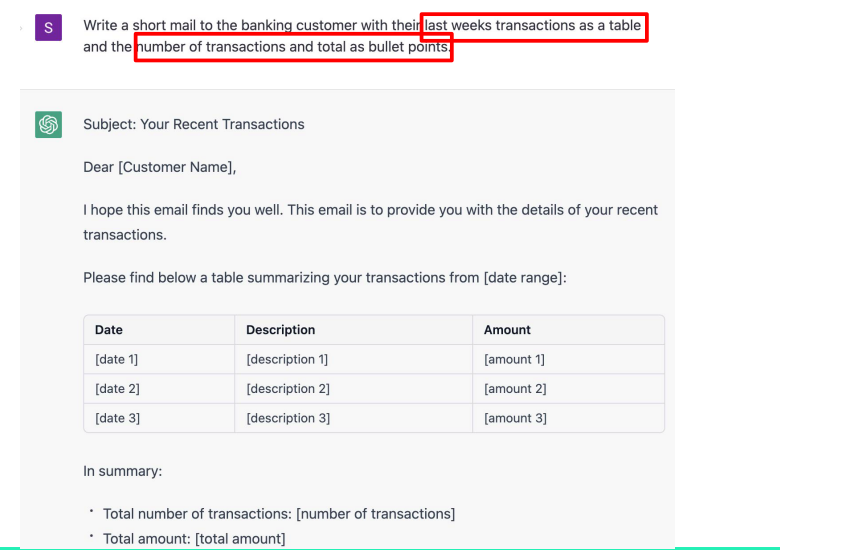
\includegraphics[width=0.8\linewidth,keepaspectratio]{promptengg18}

{\tiny (Ref: Prompt Engineering Sudalai Rajkumar)}

\end{center}		
	
\end{frame}

%%%%%%%%%%%%%%%%%%%%%%%%%%%%%%%%%%%%%%%%%%%%%%%%%%%%%%%%%%%
\begin{frame}[fragile]\frametitle{Audience Control}

Specify the desired audience.

\begin{center}
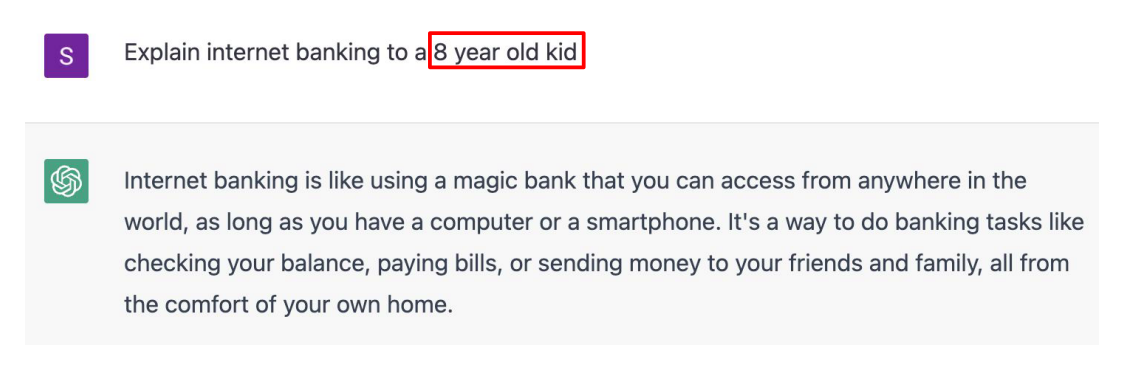
\includegraphics[width=\linewidth,keepaspectratio]{promptengg19}

{\tiny (Ref: Prompt Engineering Sudalai Rajkumar)}

\end{center}		

\end{frame}

%%%%%%%%%%%%%%%%%%%%%%%%%%%%%%%%%%%%%%%%%%%%%%%%%%%%%%%%%%%
\begin{frame}[fragile]\frametitle{Context Control}

Specify the information about the context.

\begin{center}
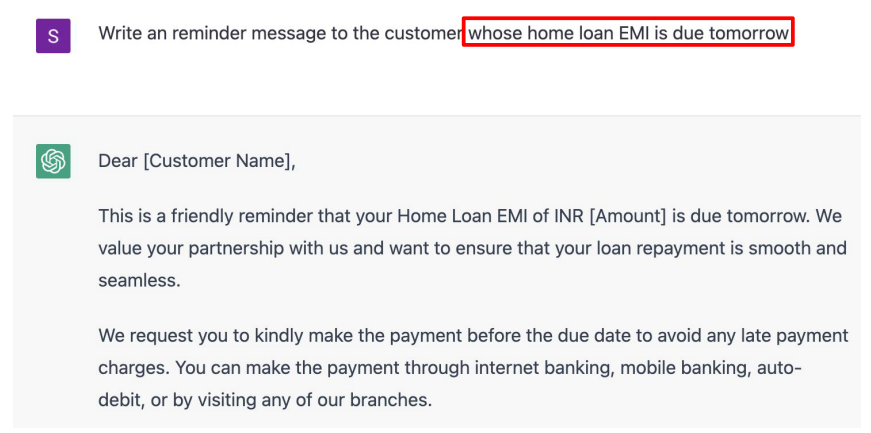
\includegraphics[width=\linewidth,keepaspectratio]{promptengg20}

{\tiny (Ref: Prompt Engineering Sudalai Rajkumar)}

\end{center}		

\end{frame}





% %%%%%%%%%%%%%%%%%%%%%%%%%%%%%%%%%%%%%%%%%%%%%%%%%%%%%%%%%%%
% \begin{frame}[fragile]\frametitle{Prompting by Examples}

% \begin{center}
% 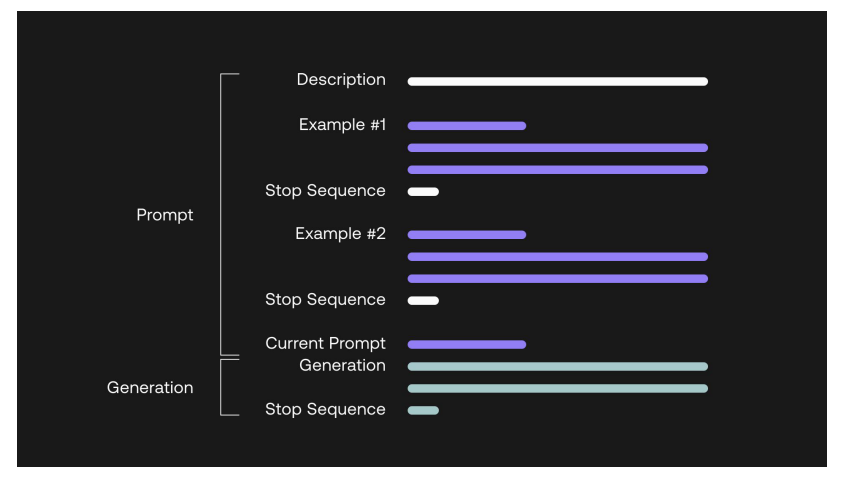
\includegraphics[width=\linewidth,keepaspectratio]{promptengg8}

% {\tiny (Ref: Cohere https://txt.cohere.ai/generative-ai-part-1/)}

% \end{center}		
		


% \end{frame}

% %%%%%%%%%%%%%%%%%%%%%%%%%%%%%%%%%%%%%%%%%%%%%%%%%%%%%%%%%%%
% \begin{frame}[fragile]\frametitle{Prompting by Examples}

% \begin{center}
% 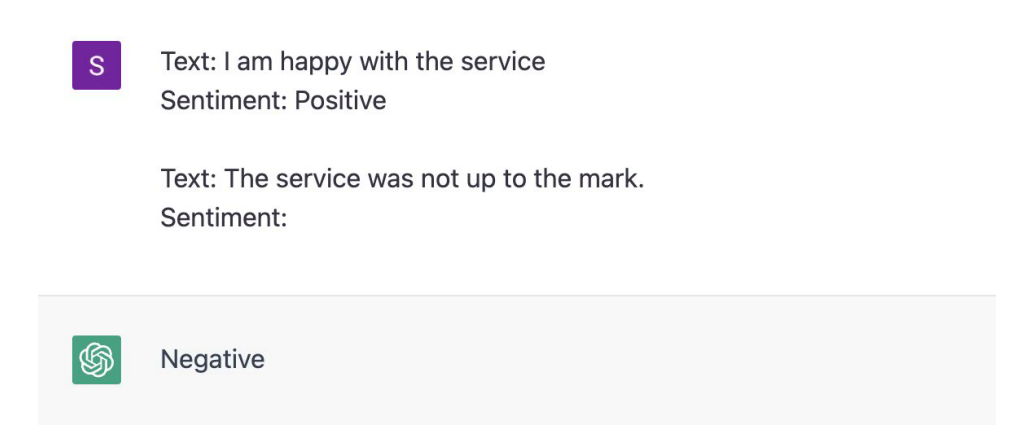
\includegraphics[width=\linewidth,keepaspectratio]{promptengg9}

% {\tiny (Ref: Cohere https://txt.cohere.ai/generative-ai-part-1/)}

% \end{center}		
		
% \end{frame}

% %%%%%%%%%%%%%%%%%%%%%%%%%%%%%%%%%%%%%%%%%%%%%%%%%%%%%%%%%%%
% \begin{frame}[fragile]\frametitle{Principles or Prompt Engineering}

% \begin{itemize}
% \item Give clear and specific instructions
% \item Give the model time/steps to ``think''
% \end{itemize}
		
% {\tiny (Ref: ChatGPT Prompt Engineering for Developers - Deep Learning AI)}
		
% \end{frame}


%%%%%%%%%%%%%%%%%%%%%%%%%%%%%%%%%%%%%%%%%%%%%%%%%%%%%%%%%%%
\begin{frame}[fragile]\frametitle{Zero-shot Prompting}

\begin{itemize}
  \item \textbf{Definition}
    \begin{itemize}
      \item Zero-shot learning: Task given to the model without specific output examples.
      \item No prior examples indicating the desired output.
    \end{itemize}

  \item \textbf{Example Scenario}
    \begin{itemize}
      \item Input: A sentence without examples.
      \item Task: Model predicts sentiment of the given sentence.
    \end{itemize}

  \item \textbf{Illustrative Example (DAIR-AI)}
    \begin{itemize}
      \item \textbf{Prompt:} Classify the text into neutral, negative, or positive.
      \item \textbf{Text:} I think the vacation is okay.
      \item \textbf{Output:} Neutral
    \end{itemize}
\end{itemize}

\end{frame}

%%%%%%%%%%%%%%%%%%%%%%%%%%%%%%%%%%%%%%%%%%%%%%%%%%%%%%%%%%%
\begin{frame}[fragile]\frametitle{Few-shot Prompting}

\begin{itemize}
  \item \textbf{Definition}
    \begin{itemize}
      \item Few-shot learning: Model provided with a small number of quality examples (input and desired output).
      \item Helps the model better understand human intention and criteria for accurate outputs.
    \end{itemize}

  \item \textbf{Comparison with Zero-shot Learning}
    \begin{itemize}
      \item Few-shot learning often yields better performance compared to zero-shot learning.
      \item However, may consume more tokens and encounter context length limitations for long input/output text.
    \end{itemize}

  \item \textbf{Application in Large Language Models (e.g., GPT-3)}
    \begin{itemize}
      \item LLMs excel in zero-shot capabilities but may face performance issues in complex tasks.
      \item Few-shot learning enhances performance by offering in-context learning through task-specific examples.
    \end{itemize}

\end{itemize}

\end{frame}

%%%%%%%%%%%%%%%%%%%%%%%%%%%%%%%%%%%%%%%%%%%%%%%%%%%%%%%%%%%
\begin{frame}[fragile]\frametitle{Few-shot Prompting}

\begin{itemize}

  \item \textbf{Example Scenario (Brown et al.)}
    \begin{itemize}
      \item \textbf{Prompt:}
        \begin{itemize}
          \item A "whatpu" is a small, furry animal native to Tanzania.
          \item Example sentence: We were traveling in Africa and we saw these very cute whatpus.
          \item To do a "farduddle" means to jump up and down really fast.
          \item Example sentence: When we won the game, we all started to farduddle in celebration.
        \end{itemize}
      \item \textbf{Output:}
        \begin{itemize}
          \item The model, given one example, generates the answer for the next.
        \end{itemize}
    \end{itemize}
\end{itemize}

\end{frame}


%%%%%%%%%%%%%%%%%%%%%%%%%%%%%%%%%%%%%%%%%%%%%%%%%%%%%%%%%%%
\begin{frame}[fragile]\frametitle{Chain-of-Thought (CoT) Prompting}

\begin{itemize}
  \item \textbf{Introduction}
    \begin{itemize}
      \item CoT Prompting introduced in Wei et al. (2022).
      \item Enables LLM to tackle complex tasks by breaking them down into constituent steps.
      \item Complex reasoning through intermediate reasoning steps.
    \end{itemize}

  \item \textbf{Combining with Few-shot Prompting}
    \begin{itemize}
      \item Combine with few-shot prompting for better results on complex tasks.
      \item Requires reasoning before responding.
    \end{itemize}

\end{itemize}

\end{frame}

%%%%%%%%%%%%%%%%%%%%%%%%%%%%%%%%%%%%%%%%%%%%%%%%%%%%%%%%%%%
\begin{frame}[fragile]\frametitle{Chain-of-Thought (CoT) Prompting}


\begin{center}
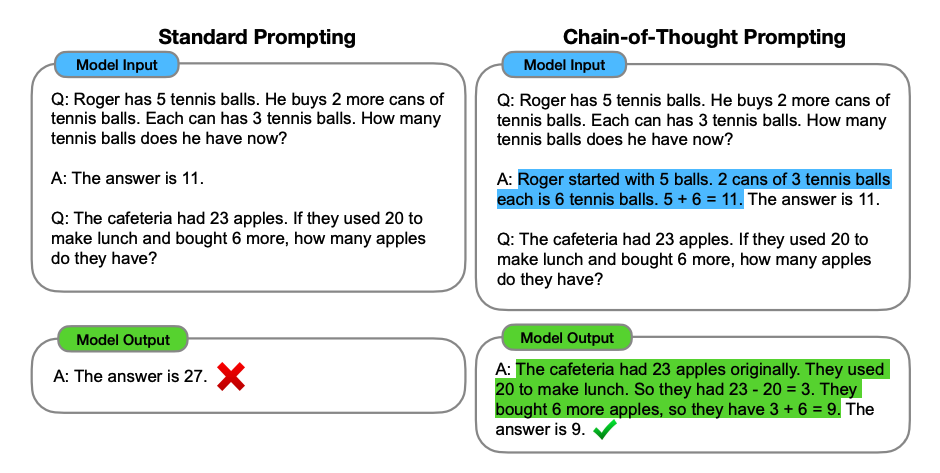
\includegraphics[width=\linewidth,keepaspectratio]{llm_prompt_cot}

{\tiny (Ref: Primers • Prompt Engineering - Aman AI)}

\end{center}				
			

\end{frame}

%%%%%%%%%%%%%%%%%%%%%%%%%%%%%%%%%%%%%%%%%%%%%%%%%%%%%%%%%%%
\begin{frame}[fragile]\frametitle{Zero-shot CoT Prompting}



    \begin{itemize}
      \item Zero-shot CoT introduced by Kojima et al. (2022).
      \item Involves appending "Let's think step by step" to the prompt.
      \item Aims to improve model performance.
    \end{itemize}

\end{frame}

%%%%%%%%%%%%%%%%%%%%%%%%%%%%%%%%%%%%%%%%%%%%%%%%%%%%%%%%%%%
\begin{frame}[fragile]\frametitle{Without Zero-shot CoT Prompting}

\begin{lstlisting}
Prompt: I went to the market and bought 10 apples. I gave 2 apples to the neighbor and 2 to the repairman. I then went and bought 5 more apples and ate 1. How many apples did I remain with?

Response: 11 apples
\end{lstlisting}


\end{frame}


%%%%%%%%%%%%%%%%%%%%%%%%%%%%%%%%%%%%%%%%%%%%%%%%%%%%%%%%%%%
\begin{frame}[fragile]\frametitle{With Zero-shot CoT Prompting}


\begin{lstlisting}
Prompt: I went to the market and bought 10 apples. I gave 2 apples to the neighbor and 2 to the repairman. I then went and bought 5 more apples and ate 1. How many apples did I remain with?

Let's think step by step.

First, you started with 10 apples.
You gave away 2 apples to the neighbor and 2 to the repairman, so you had 6 apples left.
Then you bought 5 more apples, so now you had 11 apples.
Finally, you ate 1 apple, so you would remain with 10 apples.
\end{lstlisting}


\end{frame}


%%%%%%%%%%%%%%%%%%%%%%%%%%%%%%%%%%%%%%%%%%%%%%%%%%%%%%%%%%%
\begin{frame}[fragile]\frametitle{Zero-shot CoT Prompting}

\begin{itemize}
  \item \textbf{Overview}
    \begin{itemize}
      \item CoT prompting generates reasoning chains without additional training.
      \item Sequence of short sentences with an explanation and prediction pair.
      \item No need for extra training or fine-tuning.
    \end{itemize}

  \item \textbf{Benefits}
    \begin{itemize}
      \item Step-by-step reasoning logic leading to the final answer.
      \item Particularly beneficial for complex reasoning tasks and larger models.
    \end{itemize}
\end{itemize}

\end{frame}

%%%%%%%%%%%%%%%%%%%%%%%%%%%%%%%%%%%%%%%%%%%%%%%%%%%%%%%%%%%
\begin{frame}[fragile]\frametitle{Few-shot CoT Prompting}

Few-shot CoT allows the model to view a few demonstrations of high-quality reasoning chains.

\begin{lstlisting}
Tom and Elizabeth have a competition to climb a hill.
Elizabeth takes 30 minutes to climb the hill.
Tom takes four times as long as Elizabeth does to climb the hill.
How many hours does it take Tom to climb up the hill?

Answer:

It takes Tom 30*4 = <<30*4=120>>120 minutes to climb the hill.
It takes Tom 120/60 = <<120/60=2>>2 hours to climb the hill.
So the answer is 2.

\end{lstlisting} % Placeholder for the answer, not provided in the original content.


\end{frame}

%%%%%%%%%%%%%%%%%%%%%%%%%%%%%%%%%%%%%%%%%%%%%%%%%%%%%%%%%%%
\begin{frame}[fragile]\frametitle{Few-shot CoT Prompting}

\begin{lstlisting}
Jack is a soccer player. He needs to buy two pairs of socks and a pair of soccer shoes.
Each pair of socks cost $9.50, and the shoes cost $92.
Jack has $40. How much more money does Jack need?

Answer:
The total cost of two pairs of socks is $9.50 x 2 = $<<9.5*2=19>>19.
The total cost of the socks and the shoes is $19 + $92 = $<<19+92=111>>111.
Jack needs $111 - $40 = $<<111-40=71>>71 more.
So the answer is 71.

Question:
Marty has 100 centimeters of ribbon that he must cut into 4 equal parts.
Each of the cut parts must be divided into 5 equal parts.
How long will each final cut be?

Answer:
\end{lstlisting} % Placeholder for the answer, not provided in the original content.


\end{frame}





%%%%%%%%%%%%%%%%%%%%%%%%%%%%%%%%%%%%%%%%%%%%%%%%%%%%%%%%%%%
\begin{frame}[fragile]\frametitle{Chain-of-Thought (CoT) Prompting Example}


\begin{lstlisting}[language=python]
The odd numbers add up to an even number: 4, 8, 9, 15, 12, 2, 1.
A: Adding odd numbers (9, 15, 1) gives 25. The answer is False.

The odd numbers add up to an even number: 17,  10, 19, 4, 8, 12, 24.
A: Adding odd numbers (17, 19) gives 36. The answer is True.

The odd numbers add up to an even number: 16,  11, 14, 4, 8, 13, 24.
A: Adding odd numbers (11, 13) gives 24. The answer is True.

The odd numbers add up to an even number: 17,  9, 10, 12, 13, 4, 2.
A: Adding odd numbers (17, 9, 13) gives 39. The answer is False.

The odd numbers add up to an even number: 15, 32, 5, 13, 82, 7, 1.
A:

Adding all the odd numbers (15, 5, 13, 7, 1) gives 41. 
The answer is False.

Wow! We can see a perfect result when we provided the reasoning step. 
In fact, we can solve this task by providing even fewer examples, 
i.e. just one example seems enough ...
\end{lstlisting}

\end{frame}


%%%%%%%%%%%%%%%%%%%%%%%%%%%%%%%%%%%%%%%%%%%%%%%%%%%%%%%%%%%
\begin{frame}[fragile]\frametitle{Chain-of-Thought (CoT) Prompting Example (Contd.)}



\begin{lstlisting}[language=python]
The odd numbers add up to an even number: 4, 8, 9, 15, 12, 2, 1.
A: Adding odd numbers (9, 15, 1) gives 25. The answer is False.

The odd numbers add up to an even number: 15, 32, 5, 13, 82, 7, 1. 
A:


Adding all the odd numbers (15, 5, 13, 7, 1) gives 41. 
The answer is False.

Keep in mind that the authors claim that this is an emergent ability that arises with sufficiently large language models.

\end{lstlisting}



\end{frame}


% %%%%%%%%%%%%%%%%%%%%%%%%%%%%%%%%%%%%%%%%%%%%%%%%%%%%%%%%%%%
% \begin{frame}[fragile]\frametitle{Few-shot CoT Prompting}


% \begin{center}
% 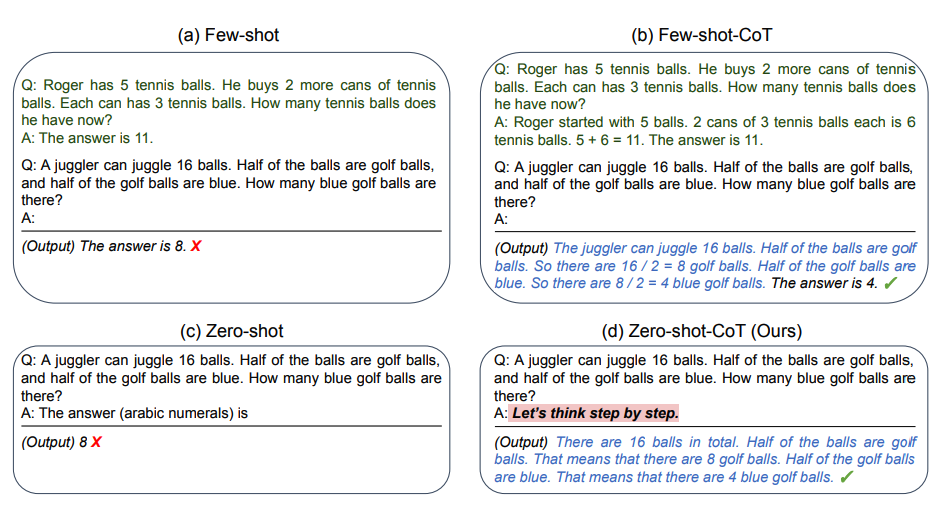
\includegraphics[width=\linewidth,keepaspectratio]{llm_prompt_zero_cot}

% {\tiny (Ref: Primers • Prompt Engineering - Aman AI)}

% \end{center}				
			

% \end{frame}



% %%%%%%%%%%%%%%%%%%%%%%%%%%%%%%%%%%%%%%%%%%%%%%%%%%%%%%%%%%%
% \begin{frame}[fragile]\frametitle{Automatic Chain-of-Thought (Auto-CoT)}


% \begin{center}
% 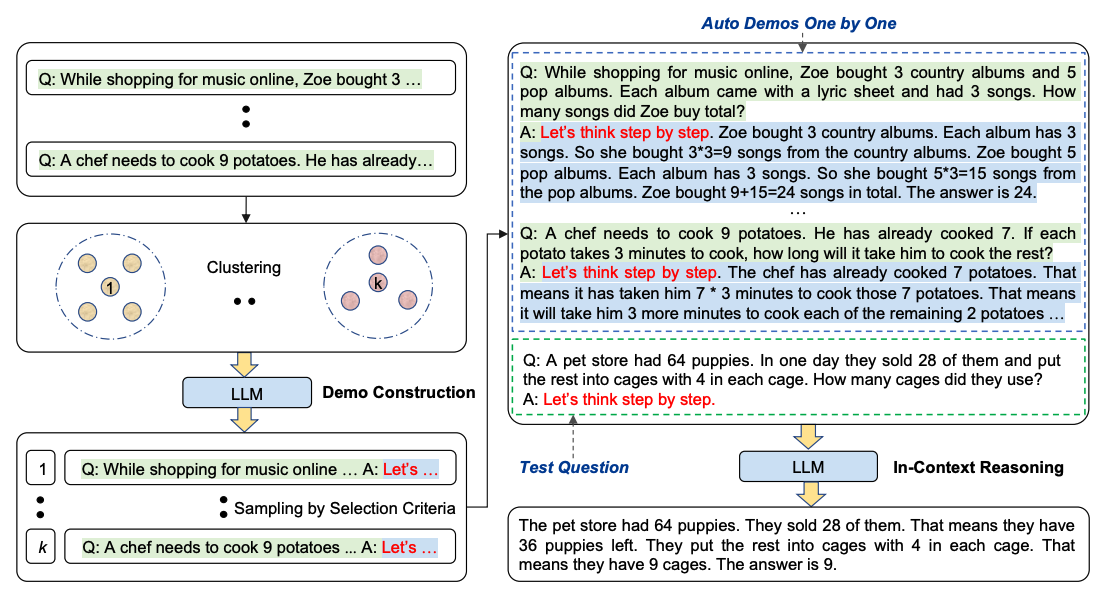
\includegraphics[width=\linewidth,keepaspectratio]{llm_prompt_auto_cot}

% {\tiny (Ref: Primers • Prompt Engineering - Aman AI)}

% \end{center}				
			

% \end{frame}

% %%%%%%%%%%%%%%%%%%%%%%%%%%%%%%%%%%%%%%%%%%%%%%%%%%%%%%%%%%%%%%%%%%%%%%%%%%%%%%%%%%
% \begin{frame}[fragile]\frametitle{Automatic Chain-of-Thought (Auto-CoT)}

% \begin{itemize}
  % \item \textbf{Introduction}
    % \begin{itemize}
      % \item Applying chain-of-thought prompting with demonstrations involves hand-crafting examples, which can be suboptimal.
      % \item Zhang et al. (2022) propose Auto-CoT to eliminate manual efforts by leveraging LLMs.
      % \item Uses the "Let’s think step by step" prompt to generate reasoning chains for demonstrations automatically.
    % \end{itemize}

  % \item \textbf{Automatic Process}
    % \begin{itemize}
      % \item Automatic process may still have mistakes in generated chains.
      % \item Diversity of demonstrations is crucial to mitigate the effects of mistakes.
    % \end{itemize}

  % \item \textbf{Auto-CoT Stages}
    % \begin{itemize}
      % \item \textbf{Stage 1: Question Clustering}
        % \begin{itemize}
          % \item Partition questions of a given dataset into a few clusters.
        % \end{itemize}

      % \item \textbf{Stage 2: Demonstration Sampling}
        % \begin{itemize}
          % \item Select a representative question from each cluster.
          % \item Generate its reasoning chain using Zero-Shot-CoT with simple heuristics.
        % \end{itemize}
    % \end{itemize}

  % \item \textbf{Simple Heuristics}
    % \begin{itemize}
      % \item Length of questions (e.g., 60 tokens).
      % \item Number of steps in rationale (e.g., 5 reasoning steps).
      % \item Encourages the model to use simple and accurate demonstrations.
    % \end{itemize}
% \end{itemize}

% \end{frame}

%%%%%%%%%%%%%%%%%%%%%%%%%%%%%%%%%%%%%%%%%%%%%%%%%%%%%%%%%%%%%%%%%%%%%%%%%%%%%%%%%%
\begin{frame}[fragile]\frametitle{}
\begin{center}
{\Large Sample (Simple) Gen AI Applications of Prompts}
\end{center}
\end{frame}

%%%%%%%%%%%%%%%%%%%%%%%%%%%%%%%%%%%%%%%%%%%%%%%%%%%%%%%%%%%
\begin{frame}[fragile]\frametitle{Text Generation}

\begin{center}
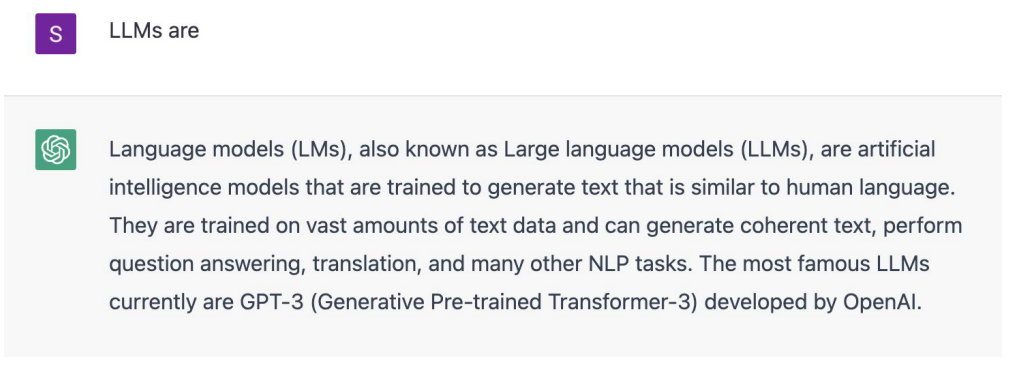
\includegraphics[width=\linewidth,keepaspectratio]{promptengg10}

{\tiny (Ref: Prompt Engineering Sudalai Rajkumar)}

\end{center}		
		


\end{frame}

%%%%%%%%%%%%%%%%%%%%%%%%%%%%%%%%%%%%%%%%%%%%%%%%%%%%%%%%%%%
\begin{frame}[fragile]\frametitle{Text Classification}

\begin{center}
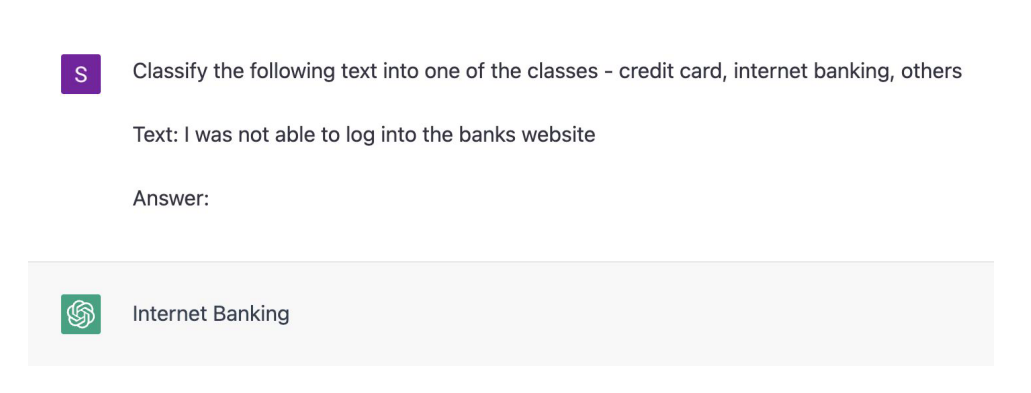
\includegraphics[width=\linewidth,keepaspectratio]{promptengg11}

{\tiny (Ref: Prompt Engineering Sudalai Rajkumar)}

\end{center}		
		


\end{frame}

%%%%%%%%%%%%%%%%%%%%%%%%%%%%%%%%%%%%%%%%%%%%%%%%%%%%%%%%%%%
\begin{frame}[fragile]\frametitle{Text Translation}

\begin{center}

\includegraphics[width=\linewidth,keepaspectratio]{promptengg12}

{\tiny (Ref: Prompt Engineering Sudalai Rajkumar)}

\end{center}		
		


\end{frame}

%%%%%%%%%%%%%%%%%%%%%%%%%%%%%%%%%%%%%%%%%%%%%%%%%%%%%%%%%%%
\begin{frame}[fragile]\frametitle{Text Comprehension}

\begin{center}
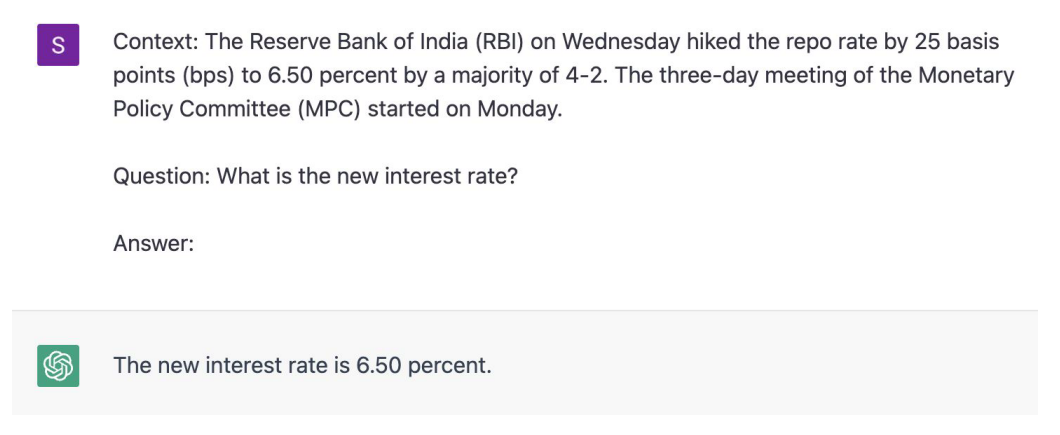
\includegraphics[width=\linewidth,keepaspectratio]{promptengg13}

{\tiny (Ref: Prompt Engineering Sudalai Rajkumar)}

\end{center}		
		


\end{frame}

%%%%%%%%%%%%%%%%%%%%%%%%%%%%%%%%%%%%%%%%%%%%%%%%%%%%%%%%%%%
\begin{frame}[fragile]\frametitle{Text Summarization}

\begin{center}

\includegraphics[width=\linewidth,keepaspectratio]{promptengg14}

{\tiny (Ref: Prompt Engineering Sudalai Rajkumar)}

\end{center}		
		


\end{frame}

%%%%%%%%%%%%%%%%%%%%%%%%%%%%%%%%%%%%%%%%%%%%%%%%%%%%%%%%%%%
\begin{frame}[fragile]\frametitle{Image Generation}

\begin{center}
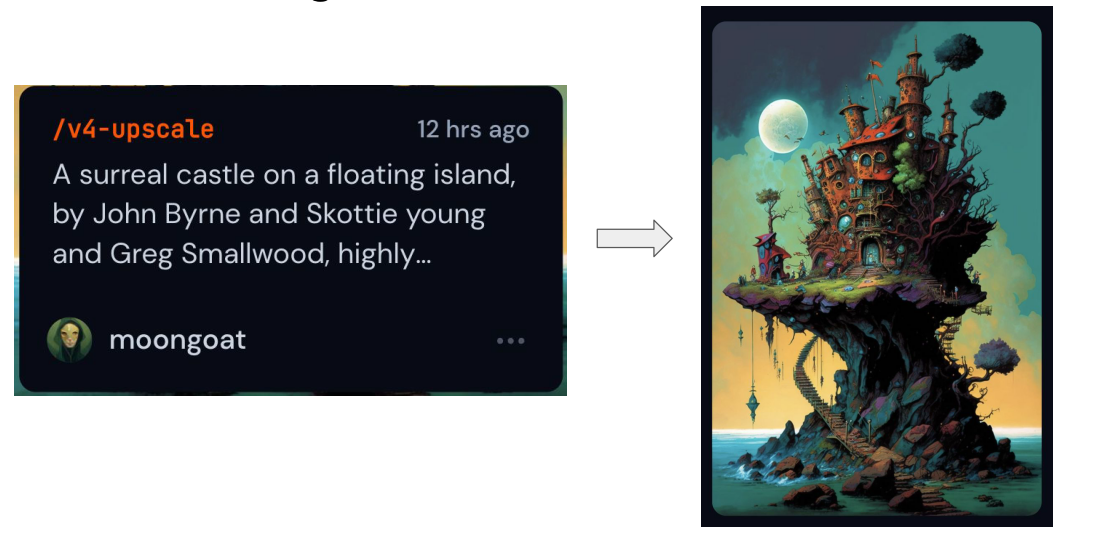
\includegraphics[width=\linewidth,keepaspectratio]{promptengg15}

{\tiny (Ref: Prompt Engineering Sudalai Rajkumar)}

\end{center}		
		
		
Models / Tools: Dall-E , Midjourney, Stable Diffusion



\end{frame}


%%%%%%%%%%%%%%%%%%%%%%%%%%%%%%%%%%%%%%%%%%%%%%%%%%%%%%%%%%%
\begin{frame}[fragile]\frametitle{For generating code using Codex}

Provide Codex with a prompt consisting of the following:



\begin{itemize}
\item  High level task description: Tell the model to use a helpful tone when outputting natural language
\item  High level context: Describe background information like API hints and database schema to help the model understand the task
\item  Examples: Show the model examples of what you want
\item  User input: Remind the model what the user has said before
\end{itemize}	 

{\tiny (Ref: https://microsoft.github.io/prompt-engineering/)}

\end{frame}


%%%%%%%%%%%%%%%%%%%%%%%%%%%%%%%%%%%%%%%%%%%%%%%%%%%%%%%%%%%
\begin{frame}[fragile]\frametitle{Programmatic Calling of Prompt}

\begin{lstlisting}
import openai
import os

from dotenv import load_dotenv, find_dotenv
_ = load_dotenv(find_dotenv())

openai.api_key  = os.getenv('OPENAI_API_KEY') # for langchain it does it automatically

def get_completion(prompt, model="gpt-3.5-turbo"):
    messages = [{"role": "user", "content": prompt}]
    response = openai.ChatCompletion.create(
        model=model,
        messages=messages,
        temperature=0, # this is the degree of randomness of the model's output
    )
    return response.choices[0].message["content"]
\end{lstlisting}
		
\end{frame}

